\documentclass{article}
\usepackage[utf8]{inputenc}
\usepackage[english]{babel}
\usepackage{todonotes}
\usepackage{float}
\usepackage{tikz}
\usepackage{rotating}
\usepackage{tikz,fullpage}
\usetikzlibrary{arrows,%
                petri,%
                topaths}%
\usepackage{tkz-berge}
\usepackage{amsmath}
\usepackage{ stmaryrd }

\title{From logic-based to algebra-based specification of geo-analytical workflows}
\author{Stan van Meerendonk }
\date{May 2020}

\tikzstyle{qgre}=[rectangle, draw, thin,fill=blue!10, scale=0.8,minimum width=1cm,inner sep=5pt]
\tikzstyle{s_square}=[rectangle,draw,thin, scale=0.8, minimum width=1cm,inner sep=5pt]

\tikzstyle{conversion}=[rectangle, draw, thin,fill=yellow!10, scale=0.8,minimum width=1cm,inner sep=5pt]

\begin{document}

%----------------------------------------------------------------------------------------
%	TITLE PAGE
%----------------------------------------------------------------------------------------

\begin{titlepage} % Suppresses displaying the page number on the title page and the subsequent page counts as page 1
	\newcommand{\HRule}{\rule{\linewidth}{0.5mm}} % Defines a new command for horizontal lines, change thickness here
	
	\center % Centre everything on the page
	
	%------------------------------------------------
	%	Headings
	%------------------------------------------------
	
	
	\begin{figure}
	    \centering
	    \includegraphics[width=8cm]{Uu_Logo.PNG}
	\end{figure}
	\smallskip
	%\textsc{\LARGE Utrecht University }\\[1.5cm] % Main heading such as the name of your university/college
	
	\textsc{\Large Master Thesis}\\[0.5cm] % Major heading such as course name
	
	%\textsc{\large Master Thesis}\\[0.5cm] % Minor heading such as course title
	
	%------------------------------------------------
	%	Title
	%------------------------------------------------
	
	\HRule\\[0.4cm]
	
	{\huge\bfseries From logic-based to algebra-based specification of geo-analytical workflows}\\[0.4cm] % Title of your document
	
	\HRule\\[1.5cm]
	
	%------------------------------------------------
	%	Author(s)
	%------------------------------------------------
	
	\large
	\textit{Author}: Stan van Meerendonk\\
	\textit{Program}: Artificial Intelligence\\
    \vspace{5 mm}
	\textit{Supervisors}\\
	Dr. A.L. Lamprecht\\
	Dr. S.W.B. Prasetya
	
%	\begin{minipage}{0.4\textwidth}
%		\begin{flushleft}
%			\large
%			\textit{Author}\\
%			B.J. \textsc{Blazkowicz} % Your name
%		\end{flushleft}
%	\end{minipage}
%	~
%	\begin{minipage}{0.4\textwidth}
%		\begin{flushright}
%%			\large
%			\textit{Supervisor}\\
%			Dr. Caroline \textsc{Becker} % Supervisor's name
%		\end{flushright}
%	\end{minipage}
	
	% If you don't want a supervisor, uncomment the two lines below and comment the code above
	%{\large\textit{Author}}\\
	%John \textsc{Smith} % Your name
	
	%------------------------------------------------
	%	Date
	%------------------------------------------------
	
	\vfill\vfill\vfill % Position the date 3/4 down the remaining page
	
	{\large\today} % Date, change the \today to a set date if you want to be precise
	
	%------------------------------------------------
	%	Logo
	%------------------------------------------------
	
	%\vfill\vfill
	%\includegraphics[width=0.2\textwidth]{placeholder.jpg}\\[1cm] % Include a department/university logo - this will require the graphicx package
	 
	%----------------------------------------------------------------------------------------
	
	\vfill % Push the date up 1/4 of the remaining page
	
\end{titlepage}

\begin{abstract}
    To be writen
\end{abstract}
\newpage
\tableofcontents

\newpage

\section{Introduction}
Science becomes increasingly more involved with complex calculations. This forces scientists to  use computational programs to let a computer execute the calculations. A common use case is combining geographical data to create more complex maps. Calculating the livability for elderly people \cite{scheider2009ontology} is an example from the geo-analytical domain. 
%The result of this calculation can be seen in figure \ref{figure:livability}. 
This can be calculated by combining geographical data regarding noise levels (Figure \ref{figure:noisevisual}), population and facilities of the neighbourhoods like the distance to a green area (Figure \ref{figure:livability}). Calculating the livability manually  is not a trivial task. 

Usually each specific use case is a sequence of already available computational components or program functions. Such sequence of components is called a workflow. The scientific community has worked on solutions to assist scientists in creating these workflows. Workflow management systems assist the user in developing workflows. Examples of such systems include Apache Taverna \cite{wolstencroft2013taverna}, Kepler \cite{altintas2004kepler} and ArcGIS ModelBuilder \cite{allen2011getting}. Although these systems solve some of the problems scientists face, the user is required to have full knowledge of all the available tools to combine them in a correct way. 



\begin{figure}
  \centering
    \includegraphics[width=8.5cm]{result3.PNG}
    \caption{Livability map showing average distance to green areas in Amsterdam within PC4 areas }
    \label{figure:livability}
\end{figure}

To support the users with workflow composition, these workflow management systems can be integrated with workflow synthesis systems. Such system takes user created constraints and generates a possible combination of components, a workflow. A user only has to worry about specifying their intent in the workflow management system. The synthesis process handles the combining of components into workflows. 

Common input methods for workflow synthesis systems are natural language templates or visual models. DECLARE \cite{pesic2007declare} and PROPHETS \cite{Prophets} are examples of both visual modeling and natural language template based systems. In these systems, the given templates and models represent some form of predetermined temporal formula reasoning over concrete or abstract tools. Examples of this are "Use tool1" or "If tool1 is used tool2 also has to be used". Modeling systems have similar constraints represented by visual models. These temporal constraints are then used to find workflows that satisfy them.


These tools reason over tools or abstractions of those tools. The goal of this project is to take it one step further. 
How could we use input that semantically describes the goal of the workflow? This would allow us to abstractly describe the goal. Furthermore, how do we link concrete tools to such an input? Finally how do we translate such input into constraints? 


\subsection{Geo-Analytical Transformation Algebra}
This project will explore Geo-anatytical Transformation Algebra (GATA), an algebra currently being developed by the geoscience department of the University of Utrecht.
This language describes geo analytical concepts on a semantic level using relational algebra. This allows to reason over calculations without a need to specify an implementation. 

GATA is part of the research to try and solve Geo-analytical question-answering (QuAnGIS) \cite{scheider2020geo}. QuAnGIS tries to find a solution for a domain specific natural language based question. In this area GATA serves as a language that expresses the answer of a question semantically. Using GATA as an input language for workflow synthesis will lead to automatic generation of Geospastial Information Systems (GIS) workflows from a single natural language question.

GATA is used to express GIS operations in terms of operations on Geospatial concepts. The algebra consists of functions that are based on relational algebra.  

\todo[inline]{explain the project a bit more with now that gata is introduced*}

% Discuss more in dept on how gata works and what it means in it's context

% Discuss the flow of operations indept
% Any function can only be executed when all its parameters have been executed
\section{Related work }
%mention work to build upon
% show you know the state and i can make the next step
To realise this project I will build upon earlier work. Generating valid type correct workflows of tools is difficult on its own. \cite{kasalica2020semantic} have developed a framework for this problem. Their API called Automatic Pipeline Explorer (APE) takes tool annotations, type systems and user intent as input and generate type correct workflows. APE translates the problem into CNF and uses a SAT solver as reasoning engine. 

User intent is modeled using semantic Linear temporal logic (SLTL) \cite{Steffen93moduleconfiguration}. SLTL is an extension of Linear Temporal Logic (LTL) \cite{emerson1990temporal}. This extension allows to express sequences of modules or tools that need to have corresponding types. SLTL allows express constraints over a type correct sequence of tools therefore it is the input representation for APE. 
% should i mention loop free? 
%For APE to use these constraints, they need to be translated into boolean CNF formulas. \cite{Bounded_model_checking} discuss a way to use SAT solvers for bounded model checking, a technique for program verification. A necessary part of this process is to encode LTL formulas into boolean formulas. For this encoding, a program is viewed as a set of state transitions. For bounded model checking you only verify your constraints for a sequence of state transition up until a certain bound. 

%APE adopts this technique to find all workflows for a bound and then increases the bound. This approach yields all possible workflows within the max bound of the program. 
The workflow synthesis system\cite{lamprecht2010synthesis} based on the minimal modal algorithm\cite{Steffen93moduleconfiguration} works somewhat similar to APE.
%There are have been other approaches to finding valid workflows. \cite{lamprecht2010synthesis} have made a workflow synthesis system based on the minimal model algorithm of \cite{Steffen93moduleconfiguration}. 
They loosely specify the constraints on their domain using SLTL and a type system. The SLTL constraints are then used to search the synthesis domain using the minimal modal algorithm to find valid workflows.  
This algorithm has been implemented by \cite{Prophets} in the PROPHETS system.
% add other systems here


This constraint based approach for finding a valid sequence is not solely used for workflow synthesis. It shares the approach with the program synthesis domain. How to handle user intent, search space and search technique \cite{gulwani2010dimensions} are similar problems as workflow synthesis is a sub domain of program synthesis. Thus sharing some of the solutions. \cite{solar2008program} describe the Sketch language for program synthesis. Sketch translates its user intent, the sketched program, into constraints for a SAT solver. This is similar with how PROPHETS handles its user intent, the natural language templates as both try to synthesize the missing gap. 


For the complete overview of what program synthesis entails I refer to Gulwani \cite{program_synthesis}. Some techniques might seem similar to program verification as program synthesis can be seen as a generalized form of program verification \cite{gulwani2011loopfree}, \cite{verificationToSynthesis}.


Earlier mentioned approaches to workflow synthesis have been tried and tested. Multiple case studies have shown great potential. For instance, a case study \cite{kasalica2019workflow} has shown APE is effective in the domain of Geoscience. A different case study \cite{palmblad2019automated} has shown effectiveness with PROPHETS in the domain of bioinformatics. Both papers show the usage of such workflow synthesis systems. They make the usability of the respective domains easier by lowering the prerequisite knowledge of all available tools. 

\section{prerequisite knowledge}
This section will discuss the knowledge necessary to understand the rest of this thesis. First I will discuss APE, the automatic pipeline explorer. The thesis will be expanding on APE so knowledge of APE is necessary. secondly I will discuss the GATA language. I will also discuss a set notation for the summation of formulas. And finally, I will discuss a formal notation for graphs. This notation will be used to reason over GATA. 


\subsection{APE}
APE is a tool that generates workflows from user intent in a given domain. A workflow is a sequence of tools or actions that transform some given input into a certain output. An example from the image processing domain would be first rotating an image 90 degrees and then inverting all the colours. APE will generate all possible type correct workflows for a given user intent.

To be able to do this, the user needs to present a domain in the form of data taxonomy and tool annotations. The taxonomy contains the abstract and concrete data types that exist in the domain. It also hold the subtype relations between the types. An example from the figures domain would be where $rectangle$ and $circle$ are a subtype of $figure$ and $squares$ would be a subtype of $rectangle$. So if some object is a $square$ it would also be a $rectangle$ and a $figure$. 

The taxonomy is used by APE to figure out what outputs of tools can fit on what input of tools. The tool annotations contain the input and output types for each tool. Tools can have zero or more input types and one or more output types. APE will create workflows where the output of one tool will fit on the input of another and thus creating type correct workflows. To be able to reason over such sequences, APE uses SLTL as constraints for the user intent. 

% not sure how and if i should mention this here
%APE translates its SLTL formulas such that a SAT solver can reason over it.

%Discuss APE in depth, how it works, the input, the constraints, SLTL, SLTL translation to propositional formulas


\subsubsection{SLTL}

SLTL reasons over alternating sequences of types and tools (also called modules). SLTL extends the LTL formalism to the BNF that can be found in equation \ref{eq:sltl}. SLTL reasons over paths like $t_0,\ m_1,\ t_1,\ m_2,\ t_2$. Here $m_1$ is the first tool in the sequence. In this thesis I will only reason over the tool states as APE handles the type correctness of a sequence. I will simplify talking about these sequences of states by leaving out the types as the types are implicit. The previous example will then look like $m_1, m_2$.


%To define the constraints themselves, I will use the earlier introduced SLTL. Using SLTL we will be able to express relations over different states. SLTL also corresponds with the way user intent is modeled in APE. This way it easier to make comparisons between GATA constraints and native APE constraints 

\begin{equation}
    \Phi :=\ true\ |\ t_c\ |\ \neg \Phi\ |\ \Phi \wedge \Phi\ |\ \Phi \vee \Phi\ |\ <m_c> \Phi\ |\  \textbf{G} \Phi\ |\ \textbf{F} \Phi\ |\  \Phi \textbf{U} \Psi\ |\  \label{eq:sltl}
\end{equation} 

These sequences of states are called paths. SLTL reasons over potentially infinite paths. A path satisfies an SLTL constraint when that formula can be used to describe that path. 

\begin{itemize}
    \item $true$ satisfies all paths regardless of their elements.
    \item $t_c$ satisfies all paths where the first element satisfies the given $t_c$. Within APE, all subtypes of $t_c$ are also allowed.
    \item $\neg$ and $\wedge$ are interpreted as their meaning in propositional logic. The $\vee$ operator can be expressed as $\neg(\neg \Phi \wedge \neg \Phi)$ but is included to be complete.
    
    \item $<m_c> \Phi$ is satisfied by paths were the second element (and thus the first tool element) satisfies $m_c$. all sub paths must satisfy $\phi$.
    
    \item $\textbf{G}\Phi$ satisfies all paths where $\Phi$ holds globally. There is no state where $\Phi$ does not hold
    \item $\Phi \textbf{U} \Psi$ satisfies all paths where $\Phi$ holds until $\Psi$ holds in the next state. This Strong until operator guarantees that $\Psi$ at some point will be satisfied. 
    \item $\textbf{F}\Phi$ satisfies all paths where $\Phi$ becomes eventually true. It guarantees that $\Phi$ happens at least one time. This operator can be expressed in terms of \textbf{U} like $true\ \textbf{U}\ \Phi$.
    
\end{itemize}

The constraints in APE are described in SLTL. Users themselves do not directly use the SLTL to create their constraints. APE provides natural language templates that represent the given constraints. This allows users from all domains to use APE. The given constraints can be found below\\

\begin{table}[h]
    \centering
    \begin{tabular}{|p{5cm}|p{5cm}|}
        \hline
        Natural language template   & SLTL constraint  \\
        \hline
        If Tool\_1 is used, Tool\_2 has to be used subsequently & $\textbf{G}(\neg <\text{Tool\_1}>true\ |\ \textbf{XF} <\text{Tool\_2}>true$\\
        \hline
        If Tool\_1 is used, Tool\_2 cannot be used subsequently & $\textbf{G}(\neg <\text{Tool\_1}>true\ |\ \textbf{XG} \neg<\text{Tool\_2}>true$\\
        \hline
        If Tool\_1 is used, Tool\_2 must has to be used next in the sequence & $\textbf{G}(\neg <\text{Tool\_1}>true\ |\ \textbf{X} <\text{Tool\_2}>true$\\
        \hline
        Use tool Tool\_1 in the solution & $\textbf{F}<\text{Tool\_1}>true$ \\
        \hline
        Do not use tool \text{Tool\_1} in the solution & $\textbf{G} \neg <\text{Tool\_1}>true$ \\
        \hline
        Use Tool\_1 as last tool in the solution & $\textbf{F}<\text{Tool\_1}>  \&\&\ \textbf{G}(\neg <\text{Tool\_1}>true\ |\ \neg \textbf{XX} true)$\\
        \hline
    \end{tabular}
    
    \caption{The natural language templates and their SLTL constraints as used by APE }
    \label{tab:APEConstraints}
\end{table}


The goal of workflow synthesis is finding interpretations or paths that satisfies the constraints. This is similar to the approach of Bounded model checking \cite{Bounded_model_checking}. This approach tries to find a counter example sequence to prove an LTL formula does not hold. Workflow generation wants to find the sequences for which the constraints do hold. Thus we can adapt the algorithm from bounded model checking to our SLTL constraints in our SAT solver based approach. The adaption of SLTL over loop free workflows is introduced in \cite{kasalica2020semantic}. \\

In this translation the notion $\llbracket f \rrbracket^i_n$ refers to the  interpretation of the formula $f$ in the $i$-th state of a sequence of length $n$. Each proposition consists of two components, the name of the proposition $p$ and the module state in which the proposition holds $m_i$. There is a separate notion for type states $t_i$. However, these will not be used can be ignored for this thesis. The resulting formula consists of propositions like $p(m_i)$ to note which state a proposition should hold. A composed expression like $p(m_i)$ can only be true or false as a whole. The translation can be found below. 
%When a proposition $p$ should hold in a certain state, it is noted like $p(m_i)$ where $m_i$ refers to the $i$-th module state. Each  

\begin{alignat*}{2}
    &\llbracket \langle p \rangle true \rrbracket^i_n  &&:= p(m_{i+1}) \\
    &\llbracket \neg f \rrbracket^i_n &&:= \neg \llbracket f \rrbracket^i_n \\
    &\llbracket f\vee g \rrbracket^i_n &&:= \llbracket f \rrbracket^i_n \vee \llbracket g \rrbracket^i_n \\
   & \llbracket f\wedge g \rrbracket^i_n &&:=\llbracket f \rrbracket^i_n \wedge \llbracket g \rrbracket^i_n \\
   &  \llbracket \textbf{G}f \rrbracket^i_n &&:= \llbracket \textbf{G} f \rrbracket^i_n \wedge  \llbracket \textbf{G} f\rrbracket^{i+1}_n \\
    & \llbracket \textbf{F}f \rrbracket^i_n &&:= \llbracket \textbf{F} f \rrbracket^i_n \vee  \llbracket \textbf{F} f\rrbracket^{i+1}_n \\
   &  \llbracket \textbf{X}f \rrbracket^i_n &&:=  \llbracket f \rrbracket^{i+1}_n \\
   & \llbracket f \rrbracket^n_n &&:= 0
\end{alignat*}

The interpretation for a single type is left out as it is not necessary for the rest of the thesis. A simple example of such translation can be found below.

\begin{equation*}
    \llbracket \textbf{F} <example\_tool>true \rrbracket^0_2 = example\_tool(m_1) \vee example\_tool(m_2)
\end{equation*}

These translated propositional formulas can be transformed into CNF. This is the required input for the SAT solver that APE uses.  

%To find a valid interpreation  Formulas like these can be converted into CNF. 

%To be able the use this approach for SLTL formulas, it needs to be


%Constraints based on SLTL are not directly usable for an SAT solver. These constraints need to be translated to a propositional formula in CNF. SLTL formula's reason over infinite sequences thus there needs to be a







%I will define my constraints in SLTL. However APE only has support for specific SLTL formulas they supply natural language templates for. To be able to 

%translation to CNF 


\subsection{GATA}
GATA describes how to calculate a result. It is defined with a simplified relational algebra as a formal basis. It reasons over relations with zero to two keys. Any of these relations represent a core concept in Geoscience \cite{kuhn2012core}. GATA consists of a set of functions that represent operations over these relations. 
But for the synthesis, the structure of the language is more important. If a workflow has the same GATA representation as the input, they represent the same operations. To determine whether two GATA expressions are the same, we need to look at the structure of the expressions. The GATA grammar is described by the BNF shown by formula \ref{eq:gatabnf}. 


\begin{align}
    F &::= ident(P)\ |\ ident  \nonumber \\
    P &::= F\ |\ F,\ P \nonumber \\
    ident &::= String \label{eq:gatabnf}
\end{align}

The language consists of functions with one or more parameters and identifiers that represent some form of input. An example of this would be equation \ref{eq:gata1}. Here $reify$, $pi$ and $interpol$ are functions that represent a data transformation. $input$ represents the input data. In concrete examples, the input represent actual data. 

\begin{equation}
    reify\ (pi\ (interpol\ (input))) \label{eq:gata1}
\end{equation}

Furthermore, there is a finite set of functions. Each function has a specific type signature. For specific information on the GATA language and its functions I refer to the GATA specification \cite{scheider2020gata}. For this thesis I will assume the all GATA expressions are type correct. The goal is to find a workflow that is the same as the input. When the input is type correct and a workflow has the same expression, that workflow will also be type correct. 

\begin{figure}
    \centering
   
   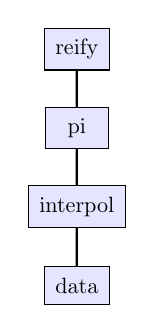
\begin{tikzpicture}
    \tikzstyle{VertexStyle}=[qgre]
  \Vertex[x=0,y=3]{reify}
  \Vertex[x=0,y=2]{pi}
  \Vertex[x=0,y=1]{interpol}
  \Vertex[x=0,y=0]{data}
  
  %\tikzstyle{EdgeStyle}=[post]
  \tikzstyle{LabelStyle}= [rectangle, draw , thin,scale=0.8]
    \Edge(reify)(pi)
    \Edge(pi)(interpol)
    \Edge(interpol)(data)
    \end{tikzpicture}
    
    \caption{The parse tree representation of expression \ref{eq:gata1}}
    \label{fig:parsetree}
\end{figure}

\subsection{Graph formalism}
Using the BNF (\ref{eq:gatabnf}) to parse GATA will create a parse tree. Figure \ref{fig:parsetree} shows the parse tree of expression \ref{eq:gata1}. The nodes in this tree are functions from the GATA language. Except for the leaves at the bottom, they only represent input data. The parse tree is build from top to bottom while pealing the most outer layer from the expression. However the data flows from bottom to top. Each function can only be applied when all its subtrees below it are applied. 
\\

To be able to use this tree as a basis for defining constraints I will use the formal definition of a graph \cite{trudeau2013introduction}.  A graph $G$ consists of a pair $(V,E)$ where $V$ is the set of vertices or nodes and $E$ is the set of edges. Each edge is a pair of nodes like $(n_1, n_2)$. When reasoning over GATA, order matters. Thus when I reason over a GATA tree, the edges are directed from top to bottom. This means that the root of the tree does not appear as the second node in an edge and the leaves do not appear as the first node in an edge. 
Using this notation the input graph I would be represented like equations \ref{eq:inputgraphexample}
 \begin{align}
     I &= (V,E) \nonumber \\
     V &= \{reify,pi,interpol, data\} \nonumber \\
     E &= \{(reify,pi), (pi,interpol), (interpol,data)\} \label{eq:inputgraphexample}
 \end{align}
 
 Finally nodes are considered unique. This holds even when different nodes represent the same function and thus have the same name. Functions can occur multiple times in the same expression. The same name appearing multiple times is not allowed in sets. However this could be circumvented by giving all nodes an id number and making the nodes a tuple of id and function name. This would increase the complexity of the given definitions and thus will be omitted. When a node is compared like $n1 == n2$ it stands for comparing the name of two different nodes instead comparing the whole nodes themselves. 
 
 
 
\\ % add that when comparing a node, we compare the name of the node and that nodes with the same name can occur multiple times. 



%Before we can start to formally define our constraints, we need to introduce the formal definition of a directed graph. A directed graph $G$ consists of a pair $(V, E)$ where $V$ is the set of vertices or nodes in the graph and $E$ is the set of arrows or directed edges. The edges consist of a pair of nodes for example $(n_1, n_2)$. I will use this graph definition to reason over GATA expressions and define constraints. GATA itself is a DAG but the difference between a DAG and a directed graph is a guarantee that cycles do not occur in the DAG. 

%\todo[inline]{The set of vertices actually should be a list. It matters for the amount of times a function appears also the workflows are lists not sets as functions can (and should be able to) appear multiple times }

%Furthermore we have a set of tools $T$. A set of annotations $A$ that exists of pairs $(t, G)$ where $t$ is a tool from the set $T$ and $G$ is a valid graph in GATA. Furthermore there is a set F that consists of all the functions currently available. I will demonstrate the constraints using equation \ref{eq:gata1} as an example running example. This graph will be mentioned as the input graph I.  

\subsection{Notations}

I will define some common notations. These notations are used throughout the thesis. The first notation I will introduce is the general set that contains all functions in the current domain, I will call this set $F$. The tools used for APE also have a GATA annotation. The set of these tool annotations will be called $A$. This set $A$ consists of pairs $(t,g)$ where $t$ is the identifier of the tool as in APE and $g$ is the tree representation of a GATA expression. Finally there is the tree that is used as input. This tree will be called $i$. I will refer to the nodes of the input tree as $V_i$ and the edges as $E_i$ These notations form the basis for reasoning about the GATA expressions with relation to the tools and input.
\\

For defining constraints, I will use set comprehension adapted from \cite{veanes2008bounded}. These set comprehensions will define sets of SLTL formulas. A BNF representing the set comprehensions can be found at \ref{eq:setcomprehensionbnf}

\begin{align}
&\textit{Basic elements}  & E::=&\ \Phi\ |\ String\ |\ Int\ |\ Boolean\ |\ Func\ |\ T \ |\ x \nonumber  \\
&\textit{Tuples} & T::=&\ ( All\ \langle,All\rangle^*)  \nonumber
\\
    &\textit{Sets of formulas}  & S ::=&\ \{\phi\ |\ F\langle,F\rangle^* \}\ |\ \emptyset\ |\ S \cup S\ |\ S\cap S\ |\ v    \nonumber\\
    &Formulas & F ::=&\ \neg F \ |\ F \wedge F\ |\ F \vee F\ |\ E == E \ |\ E \in S \ |\ E \in Func \nonumber \\
    &\textit{All types} & All ::=&\ E\ |\ S\ \nonumber\\
    &\textit{Function} & Func ::=&\ Ident( \ param\ \langle,param\rangle^*) = All \label{eq:setcomprehensionbnf}
\end{align}

The important thing to note here is that tuples can also contain sets of items. This is necessary to reason over the tool annotations. Another introduction is general use functions. Some constraints are recursively created thus introduced the need for recursive functions. The $\Phi$ in basic elements represents the SLTL structures defined earlier. Furthermore I will use a function $count$ that returns the amount of elements in the set. These set comprehensions will be used to reason over the GATA tree of the input and over the set of GATA annotations to create sets of SLTL formula's

%tuples and sets.
%tuples can have tuples and sets as basis. 
%tuples and sets can have variables and that could be tuples and sets
%variables are names that are in the <> operator of SLTL 

%maybe make the nodes a tuple of ID and name or something



%Discuss The set notation used 

%Discuss the graph, the formal definition, how it looks, how its build. 
\subsection{Relevance in AI}
This thesis is part of the research into QuAnGIS. This research aims to automatically generate workflows from natural language questions. GATA is researched as a language to capture the calculations needed to answer the natural language question. By extending APE to allow GATA as input I automate the part of the process to generate workflows from a question. QuAnGIS will benefit from the automatic generation of workflows from a GATA expression. 

%I have established a logical translation from a GATA expression to a set of constraints. These constraint 

%Discuss how this thesis will contribute to the QuAnGis, The research that tries to automate creating workflows from a natural language question. 
%Also Using a complex set of logical rules to find a solution is one way to create "intelligence" in AI 

\section{Method}
%\begin{itemize}
%    \item 
%    \item How GATA relates to APE
%    \item  
%\end{itemize}

To use GATA as constraints for APE, I need to figure out how GATA relates to a domain used by APE. In the Geo science domain GIS tools do calculations. These calculations can be described by a GATA expression. When a tool is applied all the operations in its GATA representations will be applied. Thus a workflow represents a sequence of GATA expressions. These expressions combined make a more complex expression. To use GATA as input to APE, we want workflows that represent a complex expression that need to be composed of smaller components. To be able to do this we need to find all the possible ways to break a complex expression into different smaller expressions. This has to be done in such a way that the original expression remains the same. I will use the example from \ref{eq:gata1} to explain this. 
\\

%this is the place to introduce s_i or stick to m_i from the SLTL 
First only one tool can be applied at the same time. Each time step or module state $m_i$ can only contain one tool. A tool applies a complex GATA expression. Such expression consists of one or more GATA functions that are applied in order. However with as APE uses a SAT solver to generate workflows, we can only distinguish between present (true) or not (false).  This leads to abstracting the GATA annotation of a tool from a tree to a set of applied functions. This does have as drawback that order between functions is indistinguishable.  

With this abstraction I can now determine the possible ways to separate into different states. Between states, the order should represent the original input. I will explain the example of expression \ref{eq:gata1} using the parse tree of figure \ref{fig:parsetree}. The tree is build from top to bottom but the data flows from bottom to top. This means before \textit{reify} can be applied, \textit{pi} needs to be applied. However there could also exist a tool that applies both \textit{reify} and \textit{pi}. This tool can only be applies if the \textit{interpol} has been applied. The leaves, like $data$ in this example, represent readily available input. We can ignore these data leaves when talking about the meaning of a graph as the data leaves are meaningless for the function order. These constrains results in the function separation in states that can be found in equations \ref{eq:states1}.





 

%To link tools to states or time steps, I assume only a single tool can be applied at the same time. This with the order constraint leads to a set of ways do divide the functions over states represented by equations (\ref{eq:states1}). Now we can use this example to formally start defining constraints

\begin{align}
   s0=& \{interpol,pi,reify\} &   &                 &   & \nonumber  \\
    s0=& \{interpol,pi\}          & s1=& \{reify\}    &   & \nonumber\\
    s0=& \{interpol\}             & s1=& \{pi,reify\} &   & \nonumber\\
    s0=& \{interpol\}             & s1=& \{pi\}& s2=& \{reify\} \label{eq:states1}
\end{align}

For this example I will introduce some mock-up tools to be part of the annotation set A. These tools will be used to give a concrete and concise example of the constraints. The real examples are too verbose to easily show the principle. However they will be discussed later. The tools used are shown below. The annotation set can also be found below

\begin{align}
    \text{reifyTool} &= reify(data) \nonumber \\
    \text{combinedTool} &= pi(interpol(data)) \nonumber\\
    \text{piTool} &= pi(data) \nonumber\\
    \text{interpolTool} &= interpol(data) \nonumber\\
    \text{unusedTool} &= revert(data) \label{eq:allsimpletools}
\end{align}

\begin{align}
    A =  \{ & (\text{reifyTool},& & (\{reify \} ,& \{\})&), \nonumber\\ 
    & (\text{combinedTool},& & (\{pi,interpol \} ,& \{(pi,interpol)\})&), \nonumber\\ 
    & (\text{piTool},& & (\{pi \} ,& \{\})&), \nonumber\\ 
    & (\text{interpolTool},& & (\{interpol \} ,& \{\})&),\nonumber\\ 
    & (\text{unusedTool},& & (\{revert \} ,& \{\})&)   \label{eq:toolannotations}
    &\}
\end{align}

Using this set of tools we can verify the possible workflows. There are only 2 possible workflows assuming type constraints are valid. Notice how both use a different set of tools. When we replace the tool by the set of functions the tool represents, the workflows look like one of the equations of \ref{eq:states1}.

\begin{align}
    s0=& \text{combinedTool} & s1=&\text{reifyTool} & &  \label{eq:solution1}\\
    s0=& \text{interpolTool} & s1=&\text{piTool} & s2=&\text{reifyTool} \label{eq:solution2} 
\end{align}

\subsection{Constraints}
% somewhere i should make the link from a workflow and a graph. 


Constraints are the logical rules that a workflow must comply with.
For a constraint to be usable it needs two things. It cannot exclude a correct workflow and it must be able to be calculated within reasonable time. 
A correct workflow is defined as a workflow that can be used to represent the original GATA input. A workflow can represent the input if the tools algebra related to the tools can reconstruct a graph that matches the input. The reconstruction is done in reverse order in comparison to the workflow. The last tool should represent the root function of the original gata graph. If there is a reconstructed graph that matches the original input, the workflow is deemed correct. 
To ensure this, any possible spread over states of the original input should be valid. The order of functions of the original graph should be maintained. For our example input \ref{eq:gata1}, this means one of the state equations (\ref{eq:states1}) should hold. 

To accomplish this, I first added constraints that link tools to constraints. A tool occurrence only is one time step. However a tool represents a graph. A function can only present or absent in a state. This lead to abstracting the graphs that represent a tool. Tools will only be represented by the set of functions. Now we can define a set of SLTL formulas $TA$ (Tool Annotations). This set $TA$ is expressed by equation \ref{eq:toolannotation} 

\begin{equation}
    TA = \{ \textbf{F}(t \rightarrow \bigwedge^V_{n \in V} n)\ |\ (t,(V,E))  \in A \} \label{eq:toolannotation}
\end{equation}

\begin{align*}
    TA_{example} = \{& \textbf{F}( \text{reifyTool} \rightarrow reify), &\\
    & \textbf{F}( \text{combinedTool} \rightarrow pi \wedge interpol), &\\
    & \textbf{F}( \text{piTool} \rightarrow pi), &\\
    & \textbf{F}( \text{interpolTool} \rightarrow interpol), &\\
    &\textbf{F}( \text{unusedTool} \rightarrow revert) & \}
\end{align*}

The next concern is ensuring functions are also linked to tools. The previous constraint ensures certain functions are true when a tool is true. The reverse also need to be defined. When a tool is true, one of the tools that represent is must be true. This is represented by the following constraint set TU (Tool Usage) seen in equation \ref{eq:toolusage}. It uses helper function $TF$ that returns a set of tool names that have a specific function in their annotation which can be found in equation  

\begin{align}
    TU &=  \{  \textbf{F} ( f \rightarrow \bigvee^{TF(f)}_{x \in TF(f)} x )\ |\ f \in F \} \label{eq:toolusage}\\
    TF(f) &= \{ t\ |\ f \in V, (t,(V,E))  \in A  \}
\end{align}
\begin{align*}
    TU_{example}= \{&\textbf{F} (reify \rightarrow \text{reifyTool}), &\\
    &\textbf{F} (pi \rightarrow \text{combinedTool} \vee \text{piTool}), &\\
    &\textbf{F} (interpol  \rightarrow \text{interpolTool}),& \\
    &\textbf{F} (revert  \rightarrow \text{unusedTool}) &\} 
\end{align*}

These constraints create the environment to reason over the functions. A function relates to a one of the tools and a tool relates to a set of functions. This enforces tools to be used when functions are required to be true. Thus this allows to create constraints just using functions

\subsubsection{Input Constraints}

\todo[inline]{Talk about what acceptable constraints should accomplish and the criteria for these constraints. Like "should reduce the amount of solutions without removing a correct solution" and "Should be calculable within a reasonable amount of time"}

Now that functions and tools are linked, the environment to reason about functions is created. This allows us to define constraints regarding the input. First there are two simple constraints. Later I will discuss the more complex constraints regarding the input. The first simple constraint is function usage (FU). All tools present in the input should appear in the workflow. This is represented by the set FU as can be seen in equation \ref{eq:functionusage}

%These constraints create the environment to reason over the functions. A function relates to a one of the tools and a tool relates to a set of functions. This enforces tools to be used when functions are required to be true. Thus this allows to create constraints just using functions

\begin{equation}
    FU = \{ \textbf{F}(f)\ |\ f \in V_i\ \}
    \label{eq:functionusage}
\end{equation}

\begin{align*}
    FU_{example}=\{& \textbf{F}(refiy), \\
    &\textbf{F}(pi), \\
    & \textbf{F}(interpol)& \}
\end{align*}

The last simple constraint is regarding function prevention. The meaning of a workflow would change if a function is used that is not present in the original input. To realize this I will prevent functions not present in the input to appear in the workflows. This constraint is shown by equation \ref{eq:functionprevention}

\begin{equation}
    FP = \{ \textbf{G}(\neg f)    \ |\ f \notin V_i,\ f \in F\} \label{eq:functionprevention}
\end{equation}
\begin{align*}
    FP_{example} = \{& \textbf{G}(\neg\ revert)\} 
\end{align*}


%These constraints create the environment to reason over the functions. A function relates to a one of the tools and a tool relates to a set of functions. This enforces tools to be used when functions are required to be true. Thus this allows to create constraints just using functions

% probably should move the last 2 simple tool constraints to ideal constraints


%    TA = \{ F(t -> \bigvee Vertices) | (Vertices,Edges) \in Graph | (tool,Graph)  \in Annotations \} \label{eq:toolannotation}


% This can only work after some assumptions. like a tool uses a function only once and such. 





% Talk about what acceptable constraints should accomplish and the criteria for these constraints. Like "should reduce the amount of solutions without removing a correct solution" and "Should be calculable within a reasonable amount of time"

%\todo[inline]{also talk about some of the more basic constraints as tools linked to functions and functions linked to tools}

% also talk about some of the more basic constraints as tools linked to functions and functions linked to tools

 
The next set of constraints are a bit more complex. They take the structure of the graph into account. The first constraint of this set ensures the order of the graph. This concerns the edges of the graph. As shown in figure \ref{fig:parsetree}, \textit{pi} needs to be calculated before or at the same time as \textit{reify}. This holds for the whole graph thus there is a relation for each edge. This leads to the order constraints (ORD) described by equation \ref{eq:orderconstraint}.

\begin{equation}
    ORD = \{\textbf{F}((e_2 \wedge e_1) \vee (e_2 \wedge \textbf{X} (e_1)  )\  |\  (e_1,e_2) \in  E ,\ (V,E) \in  I  \} \label{eq:orderconstraint}
\end{equation}

\begin{align*}
    ORD_{example} = \{ & \textbf{F}((interpol \wedge pi) \vee (interpol \wedge \textbf{X} (pi)  ), \\
    &\textbf{F}((pi \wedge reify) \vee (pi \wedge \textbf{X} (reify)  ) &
    \}  
\end{align*}

furthermore we can limit the amount of results by enforcing the root of the input as the last function. Any workflow where the root function is not the last function in the workflow would not satisfy the input. The last function (LF) constraint is shown by equation \ref{eq:lastfunction}. 

% this constraint is a copy of the last tool constraint of APE 
% only works because for each workflow length a 
% it basically says at some put r should be true and r can't be true unless there is nothing next

%F <Tool 1>true & G(¬ <Tool 1>true | ¬ X X true)
\begin{equation}
    LF = \{ \textbf{F} (r) \wedge \textbf{G} ( \neg\ r \vee \neg (\textbf{X X})) \ |\ r \not = e_2,\ r \in V_i,\ (e_1, e_2) \in E_i \}
    \label{eq:lastfunction}
\end{equation}

\begin{equation*}
    LF_{example} = \{ \textbf{F} (reify) \wedge \textbf{G} ( \neg\ reify \vee \neg (\textbf{X X})) \}
\end{equation*}

The last two constraints concerns the number of times a function can appear in a workflow. The first constraints enforces a function is used in exactly as many different tools as it appears in the input. This constraint is based on domain knowledge of Geoscience and on the tool examples. A tool uses a specific function only at most once. Thus when a function appears twice, tools that represent it should appear twice. Each function, the constraint is depended on how often it appears in the graph. The constraint function count (FC) is shown by equation \ref{eq:functioncount}. The helper function \textit{ generateFC} recursively generates the SLTL constraint for any length. 

For this we use the helper function \textit{generateFC} 
% However this constraint is not expressable with 

% only works when multiple occurrences may appear in the sets of the same function. 
\begin{equation}
    FC = \{   generateFC(countFn(f_1), f_1)\ |\ f_1 \in V_i\} \label{eq:functioncount}
\end{equation}
\begin{align*} 
countFn(f_1) =& count(\{ f_2\ |\ f_2 = f_1, f_2 \in V_i \})\\
    generateFC(0,f) =&\ true \\
    generateFC(i,f) =&\ \textbf{F}(f \wedge \textbf{X}\ \text{generateFC}(i-1,f))
\end{align*}

The last used constraint also regards the amount of times a function can appear. This constraint limits the amount of time a function can appear. A function should not appear more times than it appears in the graph. This leads to the function limiting constraint (\textit{FL}) that is shown by equation \ref{eq:functionlimiting}. It reuses the \textit{generateFC} function. It will prevent any combination of functions longer the amount of times it appears in the input.

\begin{equation}
    FL = \{ \textbf{G}( \neg  generateFC(countFn(f_1) +1, f_1))\ |\ f_1 \in V_i \} \label{eq:functionlimiting}
\end{equation}


Thus the complete set of constraints would look like equation \ref{eq:complete1}.

\begin{equation}
    \text{Gata constraint set}= \{TA, TU, FU, FP, ORD, LF, FC,FL\} \label{eq:complete1}
\end{equation}
 \\
 
 \todo[inline]{Maybe return to the example and show the possible workflows}
 
% if there is an edge a,b and a,c and b != c then use F else use the same or next for the future constraints 

% \begin{itemize}
%     \item Order constraint, from root to leaf
 %    \item last used constraint
%     \item cardinality constraint
 %    \item introduce functions with more than one parameter
% \end{itemize}

\subsubsection{Functions with more parameters}
\todo[inline]{Introduce a small example that has a function with more parameters and how it changes some things. order becomes less strikt}

The set of constraints from equation \ref{eq:complete1} covers the graphs that look like figure \ref{fig:parsetree}. However, functions are able to have more than a single parameter. Examples of this are the functions \textit{lotopo} and \textit{sigma}. This can be seen in equation \ref{eq:multipleparamExample} and figure \ref{fig:smallGataGraph2}. 
\begin{equation}
lotopo(pi(interpol(data1)),sigma(data2,data3)) \label{eq:multipleparamExample}
\end{equation}

Before the function \textit{lotopo} can be applied, both \textit{pi} and \textit{sigma} need to be applied. However, these functions are not dependent on each other. They are different parameters to the same instance of \textit{lotopo} and thus different parts of the graph. This leads to that the order in which \textit{pi} and \textit{sigma} are applied does not matter. However, they have to be applied before or at the same time as \textit{lotopo}. This behaviour changes the way the functions can be divided over states.

\begin{align}
   s0=& \{sigma,interpol,pi,lotopo\} &   &                 &   &   \\
   s0=& \{interpol,pi\}          & s1=& \{sigma,lotopo\}    &   &   \\
   s0=& \{sigma\}  & s1=&\{interpol,pi,lotopo \} \\
   s0=& \{sigma\} & s1=&\{ interpol\} & s2=&\{pi,lotopo \} \\
   s0=& \{sigma\} & s1=&\{ interpol,pi\} & s2=&\{lotopo \} \\
   s0=& \{interpol,pi\} & s1=&\{sigma \} & s2=&\{lotopo \} \\
   s0=& \{sigma\} & s1=&\{ interpol\} & s2=&\{pi\} & s3=&\{lotopo \} \\
   s0=&\{ interpol\}& s1=&\{pi\} &s2=& \{sigma\} & s3=&\{lotopo \}
\end{align}

 \begin{figure}
    \centering
   
   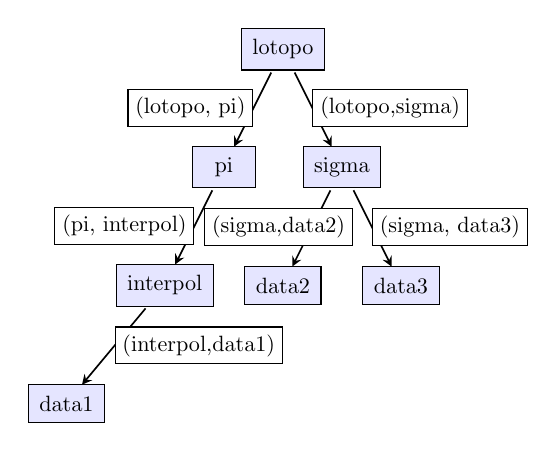
\begin{tikzpicture}
    \tikzstyle{VertexStyle}=[qgre]
  \Vertex[x=0,y=2.5]{lotopo}
  \Vertex[x=-0.75,y=1]{pi}
  \Vertex[x=0.75,y=1]{sigma}
  \Vertex[x=-1.5,y=-.5]{interpol}
  \Vertex[x=-2.75,y=-2]{data1}
  
  \Vertex[x=0,y=-.5]{data2}
  \Vertex[x=1.5,y=-.5]{data3}
  
  \tikzstyle{EdgeStyle}=[post, -stealth]
  \tikzstyle{LabelStyle}= [left, draw , thin,scale=0.8]
    \Edge[label={(lotopo, pi)}](lotopo)(pi)
    \Edge[label={(pi, interpol)}](pi)(interpol)
    
  \tikzstyle{LabelStyle}= [right , draw , thin,scale=0.8]
  \Edge[label={(interpol,data1)}](interpol)(data1)
    \Edge[label={(lotopo,sigma)}](lotopo)(sigma)
    \Edge[label={(sigma, data3)}](sigma)(data3)
    \tikzstyle{LabelStyle}= [rectangle,  draw, left=-0.52cm,  thin,scale=0.8]
    \Edge[label={(sigma,data2)}](sigma)(data2)
    
    %\draw[ultra thick,red,-stealth] (interpol) -- (0.3,0.42);
    
    \end{tikzpicture}
    
    \caption{Graphical representation of the graph of expression \ref{eq:multipleparamExample}}
    \label{fig:smallGataGraph2}
\end{figure}
 
The original order constraint is not sufficient to capture this behaviour. For functions that have multiple parameters, there is no strict ordering. To loosen the strictness of this ordering, I revise the original constraint to look like equation $ORD_{revised}$

\begin{align*}
        ORD_{rev} =\{& \{\textbf{F}((e_2 \wedge e_1) \vee (e_2 \wedge \textbf{X} (e_1)  )&  &|\ e_2 = e_3,\ (e_1,e_3) \in  E_i ,\ (e_1,e_2) \in  E_i \}, \\
        &\{\textbf{F}(e_2 \wedge \textbf{F} e_1) &  &|\ e_2 \not= e_3,\ (e_1,e_3) \in  E_i ,\ (e_1,e_2) \in  E_i\}\}
\end{align*}

\begin{align*}
    ORD_{example2} = \{& \textbf{F}(pi \wedge \textbf{F}\ lotopo), \\
    & \textbf{F}(sigma \wedge \textbf{F}\ lotopo), \\
    &\textbf{F}((interpol \wedge pi) \vee (interpol \wedge \textbf{X} (pi)  ) 
    \}
\end{align*}
The usage of \textbf{F} captures the both the order and looseness required by multiple parameter functions. Both \textit{pi} and \textit{sigma} can be used at the same time as \textit{lotopo}. If \textit{lotopo} is not used at the same time, it has to appear somewhere after. However with this solution, a workflow would still be valid when \textit{lotopo} is applied before either \textit{pi} or \textit{sigma} and it is applied again afterwards. This is not a problem. It will be solved by either the maximum usage of the function constraint or the filtering of the solutions afterwards. The constraint does lower the amount solutions while preserving the new situations. This leads to changing the constraint set to equation \ref{eq:complete2}
\begin{equation}
 \text{Gata constraint set}= \{TA, TU, FU, FP, ORD_{rev}, LF, FC,FL\} \label{eq:complete2}
\end{equation}
 
 
 %talk about the most specific constraints like completely defining a path from root to leaf and the function parameter constraint. they are the most specific but take the longest to compute. 

 %also introduce the concept of splitting the tree in all paths. 



\subsubsection{Other considered constraints}
The earlier mentioned constraint are fast to compute to CNF, however they are not precise. They do not directly describe the graph. Only parts of the graph are directly constraint. This allows for solutions to fall through the constraints that do not represent the input. To this end, I have tried to formulate more precise constraints. \\

One constraint I tested was a more precise order constraint. Each constraint would fully define a branch of the tree from the root to a leaf. When a workflow represents all possible branches, it should represent the whole tree more precise. Defining the whole tree in a single constraint would result in a unnecessary long and complex constraint. The constraint is represented by equation \ref{eq:branchConstraint} and uses the helper function \textit{generateBranches}.

\begin{equation}
    BRANCH = \{ generateBranches(l)\ |\ l \not = e_1,\ l \in V_i,\ (e_1, e_2) \in E_i \} \label{eq:branchConstraint}
\end{equation}
\begin{align*}
    generateBranches(n) = \{
    &\textbf{F}(n \wedge f)\ |\ f \in generateBranches(e_2) ,\ n = e_2 ,\ (e_1,e_2) \in E_i,\ n \in V_i \}
\end{align*}
\begin{align*}
    BRANCH_{example}=\{& \textbf{F}(interpol \wedge \textbf{F}(pi \wedge \textbf{F}(lotopo))), \\
    &\textbf{F}(sigma \wedge \textbf{F}(lotopo))  &  \}
\end{align*}
% 
These constraints keep the order of the functions. Chaining the \textbf{F} operators allows for every function in the same constraint to be applied in the same state. It allows for every function to be applied one after another. It also allows for alternation with other branches. Thus these constraints combined with a limit on function applications represent the possible combinations. There is a problem with this constraint however.

The helper functions builds the constraints recursively. Starting from each of the leaves, the function walks up each branch up to the root. This creates as many constraints as there are leaves. The constraints also don't have a fixed length. The longest constraint contains as many \textbf{F} operators as the length of the longest branch. For complex input, it would result in long \textbf{F} operator chains. 

Long \textbf{F} operator chains in the SLTL constraint result in exponential longer propositional formula constraints. The complexity the translation is $O(n^k)$ where \textit{n} is the length of the solution and \textit{k} is the amount of \textbf{F} or \textbf{G} operators. This complexity stems forth from the conversion method from SLTL to propositional formula. The \textbf{F} and \textbf{G} operators list all possible situations from state 0 to state n. This lead to too long increases in translation to CNF and lead to the exclusion of this constraint. 
\\
% actually is  4^k + 3^k + 2^k +1^k




Another constraint that was considered was expanding the constraint for multiple parameter functions. As discussed, the current constraint allows for all the parameters to be applied at some point before the function but it does not enforce it. This new constraint tries to be more precise. 
The constraint multiple parameter (\textit{MP}) can be found in equation \ref{eq:multipleParameterConstraint}

\begin{align}
     MP=\{\textbf{F}(& (e_2 \wedge \textbf{XF}(e_3 \wedge (e_1 \vee \textbf{X}(e_1)))\    \vee \nonumber \\
     &(e_3 \wedge \textbf{XF}(e_2 \wedge (e_1 \vee \textbf{X}(e_1)))  ) \ |\ e_2 \not= e_3,\ (e_1,e_3) \in  E_i ,\ (e_1,e_2) \in  E_i\}  \label{eq:multipleParameterConstraint}
\end{align}

This given constraint only handles functions with 2 parameters. The examples and the tool annotations I tested on only had functions with at most 2 parameters. Thus it was sufficient to capture the wanted behaviour. 
The behaviour it simulates is based on domain knowledge. Tool annotations could have functions with multiple parameters but did not branch. First, The two parameters are forced to be applied somewhere before the function. Only one of parameters can be at the same time as the function. The other parameter is strictly required before the function. Which of the parameters is applied first does not matter. The second parameter is required in sequence with the function. This increases the simplicity of the possible workflows as it reduces interleaving between branches. 

This leads to this constraint being more precise than $ORD_{revised}$ regarding the multiple parameter functions. The constraint is also more complex. This leads to an increase in translation time. For the examples I had the reduction in possible examples was not an enough trade-of to warrant its inclusion. Further research is required to determine its usefulness for bigger examples or on a bigger environment. \\

%\todo[inline]{Add table of results to compare the calculation times. i guess?}

%\todo[inline]{Talk about All the other considered constraints. Why they would work and why they are not included. However they could be included or used as a starting point for someone else}

%not used constraints
%\begin{itemize}
  %  \item Fully defining a path from root to leaf in a single constraint
  %  \item Completely defining that all the parameters should have come before a certain multi param function has appeared
%\end{itemize}

%These constraints would be more precise but take longer to generate CNF for.
%basically $n^t$ where \textit{n} is the amount of \textbf{F} or \textbf{G} operators and \textit{t} is the length of the solution


% talk about how the ideal constraints can be reduced to simpler constraints. They lose some of the restrictiveness they had 

%\todo[inline]{Add somewhere the conversion from SLTL To propositional so it actually is used in ape}

%\subsection{Constraint usage}




\subsection{Conversion Tools}

So far I talked about how to handle tools that do calculations. These tools have a representation in GATA. Using formulas to link the GATA representation to tools allowed to reason over the gata functions instead. This section will discuss how to handle tools without GATA annotation. These tools do not do geoscience relevant calculations. They handle data transformation instead. An example would transforming in a .csv file into the geographical data or transforming one data type to another without changing the actual data. These tools do not directly impact the meaning of the workflow and the GATA structure. But including these tools will help a user to find a workflow for their current situation. A user might not have the data in a format required for a strict workflow. In this case, a user will be able to pick an extended workflow that could handle the necessary transformation. I will discuss the implementation using the GATA constraint set from equation \ref{eq:complete2}.
\\

Now that I discussed the relevance of conversion tools, I can discuss how to include them in the environment. A conversion tool needs to have a normal APE tool annotation. This way APE includes it in the normal tool constraints. It will make sure its usage will be type correct, just like it would with any other tool. For simple inclusion, it is required that it does not have a GATA annotation. Without an annotation, the tool is not prevented from usage by the \textit{FP} constraint and usage is not forced by the \textit{FU} constraint. Thus without GATA annotation, the tool is not necessary for a workflow but can always be added. 
\\

This is enough for the first use case of a tool, where a tool read a file and load a GIS data structure. In this case, a tool needs to be put in front of a branch of the GATA structure. If we give such a tool the special function \textit{conversion}, we can see how it would fit in the tree. Figures  \ref{fig:conversionEx1} and \ref{fig:conversionEx2} show examples where data needs conversion before a function. 

In these figures, you can see the original graph is still the same. There is an empty node added but the original edges are untouched. The $ORD_{rev}$ constraint does not need to change to allow this behaviour as the edges are unchanged.  Thus a tool that needs to be applied before the first tool of a branch of the input does not cause conflicts with the current constraints
\\
%When a conversion tool is only necessary in front of a tree like in figures (\ref{fig:conversionEx1}, \ref{fig:conversionEx2}), the tool does not conflict with any of the constraints. 





%Probably the most common use case of this would be using a tool to read a file to a GIS data structure. An additional tool would be put in front of one of the branches of the tree. If we give such a tool the special function \textit{conversion}, we can see how it would fit in the tree. Figures  \ref{fig:conversionEx1} and \ref{fig:conversionEx2} show examples where data needs conversion before a function. 

 \begin{figure}[H]
    \centering
   \begin{minipage}{.45\textwidth}
   \centering
      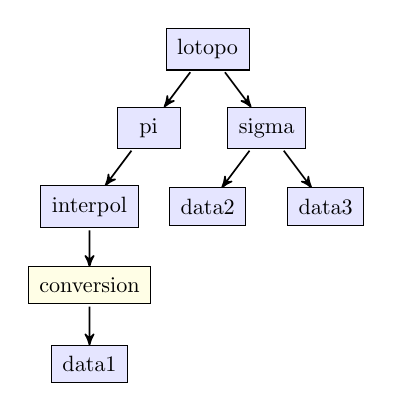
\begin{tikzpicture}
    \tikzstyle{VertexStyle}=[qgre]
  \Vertex[x=0,y=2]{lotopo}
  \Vertex[x=-0.75,y=1]{pi}
  \Vertex[x=0.75,y=1]{sigma}
  \Vertex[x=-1.5,y=0]{interpol}
  \Vertex[x=-1.5,y=-2]{data1}
  \Vertex[x=0,y=0]{data2}
  \Vertex[x=1.5,y=0]{data3}
  \tikzstyle{VertexStyle}=[conversion]
  
  \Vertex[x=-1.5,y=-1]{conversion}
  \tikzstyle{EdgeStyle}=[post]
    \Edge(lotopo)(pi)
    \Edge(pi)(interpol)
    \Edge(interpol)(conversion)
    \Edge(conversion)(data1)
    \Edge(lotopo)(sigma)
    \Edge(sigma)(data3)
    \Edge(sigma)(data2)
    \end{tikzpicture}
   
    
    \caption{Graphical representation of the graph of expression \ref{eq:multipleparamExample}. A conversion tool is used to convert \textit{data1} to input of \textit{interpol}}
    \label{fig:conversionEx1}
   \end{minipage}%
   \qquad
      \begin{minipage}{.45\textwidth}
   \centering
   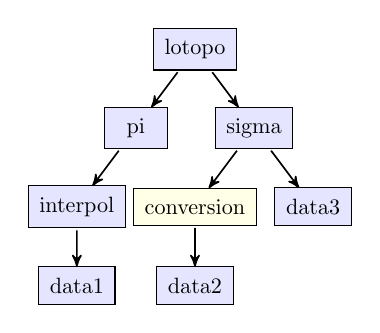
\begin{tikzpicture}
    \tikzstyle{VertexStyle}=[qgre]
  \Vertex[x=0,y=2]{lotopo}
  \Vertex[x=-0.75,y=1]{pi}
  \Vertex[x=0.75,y=1]{sigma}
  \Vertex[x=-1.5,y=0]{interpol}
  \Vertex[x=-1.5,y=-1]{data1}
  \Vertex[x=0,y=-1]{data2}
  \Vertex[x=1.5,y=0]{data3}
  \tikzstyle{VertexStyle}=[conversion]
  \Vertex[x=-0,y=0]{conversion}
  
  \tikzstyle{EdgeStyle}=[post]
    \Edge(lotopo)(pi)
    \Edge(pi)(interpol)
    \Edge(interpol)(data1)
    \Edge(lotopo)(sigma)
    \Edge(sigma)(data3)
    \Edge(sigma)(conversion)
    \Edge(conversion)(data2)
    \end{tikzpicture}
    
    \caption{Graphical representation of the graph of expression \ref{eq:multipleparamExample}. A conversion tool is used to convert \textit{data2} to input of \textit{sigma}}
   \label{fig:conversionEx2}
   \end{minipage}
\end{figure}

The last use case is when a tool converts data types in between other functions. Figures \ref{fig:conversionEx3} and\ref{fig:conversionEx4} are examples of this case. Here the edges of the original graph are changed. In figure \ref{fig:conversionEx3} the edge $(pi,interpol)$ is broken into 2 different edges with \textit{conversion} in between. This also occurs in figure \ref{fig:conversionEx4} where the edge \textit{(lotopo,sigma)} is broken in 2 edges. These examples represent edges broken up from both single and multi parameter functions. Both cases are represented differently in $ORD_{rev}$ and should be taking into account differently.



%  SPLIT BETWEEN FIGURES

 \begin{figure}[H]
    \centering
   \begin{minipage}{.45\textwidth}
   \centering
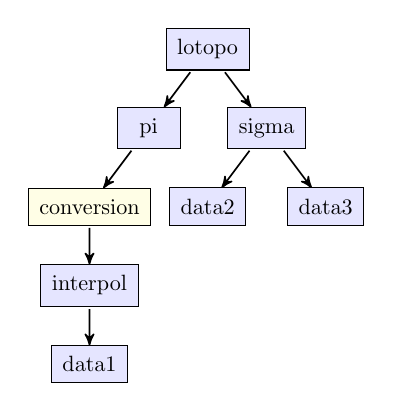
\begin{tikzpicture}
    \tikzstyle{VertexStyle}=[qgre]
  \Vertex[x=0,y=2]{lotopo}
  \Vertex[x=-0.75,y=1]{pi}
  \Vertex[x=0.75,y=1]{sigma}
  \Vertex[x=-1.5,y=-1]{interpol}
  \Vertex[x=-1.5,y=-2]{data1}
  \Vertex[x=0,y=0]{data2}
  \Vertex[x=1.5,y=0]{data3}
  \tikzstyle{VertexStyle}=[conversion]
  
  \Vertex[x=-1.5,y=0]{conversion}
  \tikzstyle{EdgeStyle}=[post]
    \Edge(lotopo)(pi)
    \Edge(pi)(conversion)
    \Edge(conversion)(interpol)
    \Edge(interpol)(data1)
    \Edge(lotopo)(sigma)
    \Edge(sigma)(data3)
    \Edge(sigma)(data2)
    \end{tikzpicture}
    
    \caption{Graphical representation of the graph of expression \ref{eq:multipleparamExample}. A conversion tool is used to convert \textit{data1} to input of \textit{interpol}}
    \label{fig:conversionEx3}
   \end{minipage}%
   \qquad
      \begin{minipage}{.45\textwidth}
   \centering
   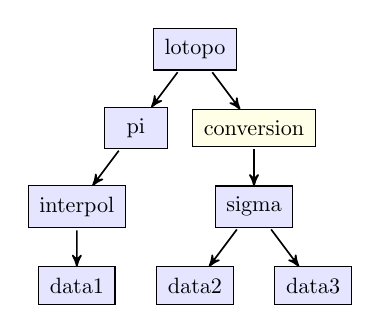
\begin{tikzpicture}
    \tikzstyle{VertexStyle}=[qgre]
  \Vertex[x=0,y=2]{lotopo}
  \Vertex[x=-0.75,y=1]{pi}
  \Vertex[x=0.75,y=0]{sigma}
  \Vertex[x=-1.5,y=0]{interpol}
  \Vertex[x=-1.5,y=-1]{data1}
  \Vertex[x=0,y=-1]{data2}
  \Vertex[x=1.5,y=-1]{data3}
  \tikzstyle{VertexStyle}=[conversion]
  \Vertex[x=0.75,y=1]{conversion}
  
  \tikzstyle{EdgeStyle}=[post]
    \Edge(lotopo)(pi)
    \Edge(pi)(interpol)
    \Edge(interpol)(data1)
    \Edge(lotopo)(conversion)
    \Edge(sigma)(data3)
    \Edge(sigma)(data2)
    \Edge(conversion)(sigma)
    \end{tikzpicture}
    
    \caption{Graphical representation of the graph of expression \ref{eq:multipleparamExample}. A conversion tool is used to convert \textit{data2} to input of \textit{sigma}}
   \label{fig:conversionEx4}
   \end{minipage}
\end{figure}

The single parameter function is represented by figure \ref{fig:conversionEx3}. To allow this behaviour we need to look at the constraint of the constraint of the edge. For the specific edge of $(pi,interpol)$ the constraint looks like $F((interpol \wedge pi) \vee (interpol \wedge X(pi))$. This constraint enforces $pi$ and $interpol$ in the same state or $interpol$ in one state and $pi$ in state directly after it. However if we want to allow a conversion tool in between these tools we also need to allow the specific case that $s0$ constains $interpol$, that $s1$ contains a conversion tool and that $s2$ containts $pi$. If we take this into account the constraint for this specific edge looks like $\textbf{F}((interpol \wedge pi) \vee (interpol \wedge \textbf{X}(pi)) \vee (interpol \wedge \textbf{X}(conversion \wedge \textbf{X}(pi))))$. This can be generalised and be used to revise the $ORD_{rev}$ constraint. The new constraint $ORD_{conv}$ can be found in equation \ref{eq:orderConversion}.
    \begin{align}
        ORD_{conv} =\{& \{\textbf{F}((e_2 \wedge e_1) \vee (e_2 \wedge \textbf{X} (e_1)\ \vee \nonumber \\ 
        &\ \ (e_2 \wedge \textbf{X}(conversion \wedge \textbf{X}(e_1)))  )&  &|\ e_2 = e_3,\ (e_1,e_3) \in  E_i ,\ (e_1,e_2) \in  E_i \}, \nonumber \\
        &\{\textbf{F}(e_2 \wedge \textbf{F} e_1) &  &|\ e_2 \not= e_3,\ (e_1,e_3) \in  E_i ,\ (e_1,e_2) \in  E_i\}\} \label{eq:orderConversion}
\end{align}
 
 However, for this constraint to be able to work, Conversion tools need to be annotated with a special tag. Otherwise I can't enforce that only conversion tools can be allowed using the $ORD_{conv}$ constraint. This $conversion$ tag needs to be included with the $TA$ and $TU$ constraints. Otherwise $conversion$ can be true without a conversion tool being used. Furthermore, the $conversion$ tag can't be included in the $FP$ constraint. As $conversion$ is never in the input, it would always be excluded. Thus $FP$ needs to be adapted to $FP_{conv}$ which can be found in equation \ref{eq:functionpreventionConv}.
 
 \begin{equation}
         FP_{conv} = \{ \textbf{G}(\neg f)    \ |\ f\not= conversion , f \notin V_i,\ f \in F\} \label{eq:functionpreventionConv}
 \end{equation}
 
 The multiple parameter function is represented by figure \ref{fig:conversionEx4}. Like with the single parameter function, I need to look at the edge and how it is represented in the constraint. For the edge of $(lotopo,sigma)$, the constraint looks like $\textbf{F}(sigma \wedge \textbf{F}(lotopo))$. This constraint already include the additional case of allowing the conversion tool. Thus for the multiple parameter functions we do not need to revise constraints. 
 
As I have shown, with minimal changes to the constraints I can allow conversion tools. Workflows will include these tools if the types of the tools in the workflow allow it.
 
 
 
 
%Discuss the necessity of the conversion tools and how/if constraints need to be adapted

%The conversion tool in the example can only occur in the beginning of 

\subsection{Graph Comparing and filtering}
Using the GATA input to generate these constraints reduces the amount of possible workflows APE is able to generate. However the constraints are not exactly compliant with the input. There might be some workflows in the resulting solutions that do not represent the input correctly. There is also the issue that in the tool annotation the ordering of the functions is discarded. This might lead to incorrect tools appearing in the resulting workflow. Tools where the correct functions are present but are in the wrong order. Thus those tools represent a different GATA expression. The use of more precise constraint comes with an increase in constraint generation time. Another approach is to filter the solutions APE returns. 
\\

% Should i create example comparisons? 
To filter solutions we need to be able to recreate a complex GATA expression from a workflow and to be able to compare the tree structure of 2 expressions. Comparing 2 trees is a relatively trivial task. You take the root of both trees and traverse to both of them in lockstep. Then compare the nodes from both trees. When one pair does not match, the trees are not equivalent. When comparing nodes, only the nodes that hold function names should be considered. The names of the data leaves are not required to be the same. These hold just a name for the relevant data. \\

To recreate a complex expression we need to look at a workflow. The root of the expression is always applied by the applied by the last tool in the workflow. A function can only be applied when its parameters are applied. Thus if we try to recreate the expression I can start from the root, the first function and the last tool. 

I will use equation \ref{eq:solution3} from the simple example to demonstrate. The GATA expression used as input is $reify(pi(interpol(input)))$ and the domain is the tool annotations from \ref{eq:toolannotation} as the domain. It shows a simple workflow of 2 tools, first use combinedTool then use reifyTool. 
\\
\begin{align}
    s0=& \text{combinedTool} & s1=&\text{reifyTool} \label{eq:solution3}
\end{align}
\begin{figure}[H]
    \centering
    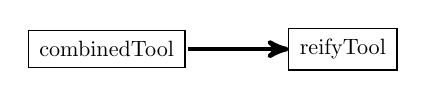
\begin{tikzpicture}
    \tikzstyle{VertexStyle}=[s_square]
        \Vertex[x=0,y=0]{combinedTool}
        \Vertex[x=3,y=0]{reifyTool}
        \tikzstyle{EdgeStyle}=[post, ultra thick]
        \Edge(combinedTool)(reifyTool)
    \end{tikzpicture}
    \caption{Visualisation of workflow found in equation \ref{eq:solution3} }
    \label{fig:my_label}
\end{figure}

To recreate the original parse tree we need to start at the outer most function. In a workflow this is always the last tool. In this case that is reifyTool. Then take the representation of the second to last tool (child tree) and combine this with the representation of the last tool (parent tree). To combine these tree, I take one leaf of the parent tree and replace this with the root of the child tree. The result of this operation can be seen in figure \ref{fig:combineGATA}

\begin{figure}[H]
    \centering
   
   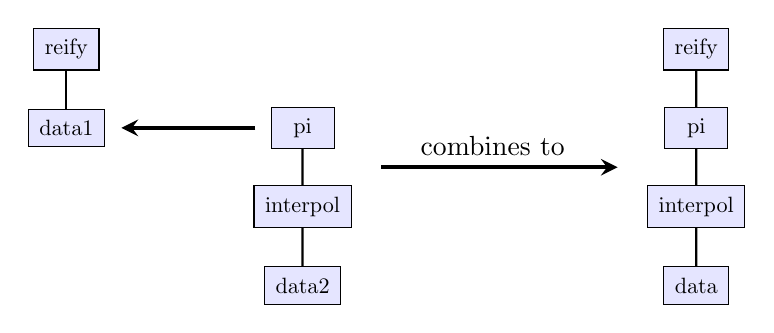
\begin{tikzpicture}
    \tikzstyle{VertexStyle}=[qgre]
  \Vertex[x=0,y=3]{reify}
  \Vertex[x=0,y=2]{data1}
  \Vertex[x=3,y=2]{pi}
  \Vertex[x=3,y=1]{interpol}
  \Vertex[x=3,y=0]{data2}
  
    \Vertex[x=8,y=3,L=reify]{reify2}
  \Vertex[x=8,y=2,L=pi]{pi2}
  \Vertex[x=8,y=1,L=interpol]{interpol2}
  \Vertex[x=8,y=0, L=data]{data3}
  
  %\tikzstyle{EdgeStyle}=[post]
  \tikzstyle{LabelStyle}= [rectangle, draw , thin,scale=0.8]
    \Edge(reify)(data1)
    \Edge(pi)(interpol)
    \Edge(interpol)(data2)
    
    \Edge(reify2)(pi2)
    \Edge(pi2)(interpol2)
    \Edge(interpol2)(data3)
    
    \draw[ultra thick,-stealth] (4,1.5) -- node [text width=2cm,midway,above ] {combines to} (7 ,1.5);
    
    \draw[ultra thick,-stealth] (2.4,2) -- (0.7 ,2);
    \end{tikzpicture}
    
    \caption{application of one tool representation to another to create the more complex expression   $reify(pi(interpol(data)))$}
  \label{fig:combineGATA}
\end{figure}

This is a simple example that only consists of two tools that have single parameter GATA representations. Usually workflows consist of more than two tools. In this case, I repeat this process from the last tool to the first tool in the workflows. Adding each new GATA representation to the accumulated graph. This creates a more complex expression that represents the workflow. When this expression is equivalent to the input expression, the workflow is a valid workflow for that input. \\

However, The process is more complex when GATA expression consists of multi parameter expressions. This increases the amount of possible combinations. If there is a function with 2 parameters, all subsequent functions have 2 possible leaves to substitute. In a situation where in a workflow of 3 tools the last tool has 2 parameters, the amount of possible solutions for this example is $2^2$. This is the amount of parameters to the power of the amount of subsequent tools left.

Each of these solutions needs to be verified until a matching solution has been found. If no matching solution can be found. The workflow is invalid and should not be considered a solution. Thus multi parameter functions exponentially increase the amount of solutions needed to be verified. However this method guarantees only valid workflows are returned as solutions. 

%\begin{itemize}
 %   \item can't capture the order of a tool, just the functions a tool consists of.
 %   \item The constraints are not strictly describing correct solutions so bad graph representations are still returned.
 %   \item describe how to build a graph 
 %   \item describe how to compare a graph 
%\end{itemize}


\section{Comparison between native APE and GATA constraints}
%To test the usefullness of the gata constraints and the filtering we compare it against the same usecases with trying to just use the constraints as defined in APE.\\

In this section I will compare using the constraints available in APE to the constraints generated by a GATA input. First I will explain the examples I will be using. Then I will compare do a metric evaluation of both approaches. Finally both approaches will be compared conceptually. 


\subsection{Examples}

For the evaluation, I will use four different examples. These examples have been prepared by Simon Scheider of the Geoscience department. The examples are increasingly complex. I will give an explanation, the GATA representation and the ape constraints of each example. For each example an example GATA expression and workflow have been prepared by Simon Scheider of the Geoscience department.

\subsubsection{Noise portion}
This is the first and most simple example. This example represents the question "Where in Amsterdam is noise more intense than 70 dB?". The target workflow consists of 5 tools and can be seen in figure \ref{figure:noisePortionworkflow}. The given GATA expression can be seen below. The tools relevant to this example can be seen in table \ref{tab:example1tools}

% Maybe ook de tools in een tabel er bij zetten

\begin{sidewaysfigure}
  \centering
    \includegraphics[width=23cm]{example1_workflow.png}
    \caption{The given workflow for the noise portion example }
    \label{figure:noisePortionworkflow}
\end{sidewaysfigure}

\begin{tabbing}    
\hspace{0.5cm}     \= \hspace{0.5cm}  \= \hspace{0.5cm}  \= \hspace{0.5cm}  \=\hspace{0.5cm}  \=\hspace{0.5cm} \= \hspace{0.5cm}  \= \hspace{0.5cm} \= \hspace{0.5cm} \= \hspace{0.5cm}\kill
reify( \\
\> pi1 ( \\
\>\>sigmale(\\
\>\>\>bowtie(\\
\>\>\>\>revert(contour\_noise),\\ 
\>\>\>\>deify(\\
\>\>\>\>\>merge(\\
\>\>\>\>\>\>pi2(\\
\>\>\>\>\>\>\>sigmae(objectregions\_muni, object\_utrect)\\
\>\>\>\>\>\>)\\
\>\>\>\>\>)\\
\>\>\>\>)\\
\>\>\>),\\
\>\>\>70\\
\>\>)\\
\>)\\
)
\end{tabbing}

\begin{table}[h]
    \centering
    \begin{tabular}{|c|c|}
        \hline
        Tool name & GATA expression  \\
        \hline
        ContourToFieldRaster & $revert (contour\_x)$\\
        \hline
        SelectLayerByAttributeObjects & $sigmae (objectregions\_x, object\_y)$\\
        \hline
        ClipField2ObjectExtent & $bowtie (field\_x, deify (merge (pi2 (objectregions\_x))))$\\
        \hline
        LocalMapAlgebraSubOrder & $sigmale (field\_x, ordinal\_y)$\\
        \hline
        RegionFromRasterExtent & $reify (pi1 (field\_x))$\\
        \hline
    \end{tabular}
    \caption{Tools required for the noise portion example}
    \label{tab:example1tools}
\end{table}
\subsubsection{Noise proportion}
The second example has the longest resulting workflows. All the solutions have 7 tools in their workflow. Figure \ref{figure:noiseProportionworkflow} is an example of this. The question this example tries to solve is "What is the proportion of the region where noise is greater than 70 dB in Amsterdam?". The GATA expression that calculates this can be seen below. The tools relevant can be found in table \ref{tab:example2tools}. A possible workflow can be seen in in figure
The GATA expression branches high in the parse tree.  This allows for a lot of variation in when a part of the expression is represented in the workflow. 

\begin{sidewaysfigure}
  \centering
    \includegraphics[width=23cm]{example2_workflow.png}
    \caption{The given workflow for the noise proportion example }
    \label{figure:noiseProportionworkflow}
\end{sidewaysfigure}
\begin{tabbing}
\hspace{0.5cm}     \= \hspace{0.5cm}  \= \hspace{0.5cm}  \= \hspace{0.5cm}  \=\hspace{0.5cm}  \=\hspace{0.5cm} \= \hspace{0.5cm}  \= \hspace{0.5cm} \= \hspace{0.5cm} \= \hspace{0.5cm}\kill
bowtie\_ratio ( \\
\>groupby\_size ( \\
\>\>sigmae (\\
\>\>\>lotopo (\\ 
\>\>\>\>pi1 (\\
\>\>\>\>\>sigmale(revert(contour\_noise), 70)\\
\>\>\>\>),\\
\>\>\>\>sigmae(objectregions\_muni, object\_Amsterdam)\\
\>\>\>),\\
\>\>\>in\\
\>\>)\\
\>),\\ 
\>groupby\_size (\\
\>\>sigmae (\\
\>\>\>lotopo (\\
\>\>\>\>deify (\\
\>\>\>\>\>merge (\\
\>\>\>\>\>\>pi2 (objectregions\_muni)\\
\>\>\>\>\>)\\
\>\>\>\>),\\
\>\>\>\>sigmae(objectregions\_muni, object\_Amsterdam)\\
\>\>\>),\\
\>\>\>in\\
\>\>)\\
\>)\\
)
\end{tabbing}

\begin{table}[h]
    \centering
    \begin{tabular}{|l|p{10.5cm}|}
        \hline
        Tool name & GATA expression  \\
        \hline
        ContourToFieldRaster & $revert (contour\_x)$\\
        \hline
        SelectLayerByAttributeObjects & $sigmae (objectregions\_x, object\_y)$\\
        \hline
        LocalMapAlgebraSubOrder & $sigmale (field\_x, ordinal\_y)$\\
        \hline
        ZonalStatisticsSize & $groupby\_size (sigmae (lotopo (pi1 (field\_x), objectregions\_y), in))$ \\
        \hline
        AddArea & 
        $\begin{array} {lcl} groupby\_size (sigmae &(lotopo (deify (merge (pi2 (objectregions\_x))), \\ & objectregions\_x), in)) \end{array}$
        \\ 
        \hline
        CalculateRatio & $bowtie\_ratio (objects\_x, objects\_y)$\\
        \hline
    \end{tabular}
    \caption{Tools required for the noise proportion example}
    \label{tab:example2tools}
\end{table}
% groupby\_size (sigmae (lotopo (deify (merge (pi2 (objectregions\_x))), objectregions\_x), in))$


\subsubsection{Object amount and distribution}

The third example has the shortest workflow. The GATA expression is relatively complex for solutions with only 3 tools as can be seen in figure \ref{figure:objectAmountWorkflow}. The question this example tries to solve is "What is the number of people for each neighborhood in Utrecht?". The GATA expression that calculates this can be seen below. The tools required can be found in table \ref{tab:example3tools} . 
%What is the neighborhood distribution of people in Utrecht?
%What is the number of people for each neighborhood in Utrecht?


\begin{sidewaysfigure}
  \centering
    \includegraphics[width=23cm]{example3_workflow.png}
    \caption{The given workflow for the Object amount and distribution example }
    \label{figure:objectAmountWorkflow}
\end{sidewaysfigure}
\begin{tabbing}
\hspace{0.5cm}     \= \hspace{0.5cm}  \= \hspace{0.5cm}  \= \hspace{0.5cm}  \=\hspace{0.5cm}  \=\hspace{0.5cm} \= \hspace{0.5cm}  \= \hspace{0.5cm} \= \hspace{0.5cm} \= \hspace{0.5cm}\kill
groupby\_sum (\\
\>bowtie* (\\
\>\>sigmae (\\
\>\>\>otopo (\\
\>\>\>\>objectregions\_households,\\
\>\>\>\>bowtie (\\
\>\>\>\>\>objectregions\_neighbourhoods,\\
\>\>\>\>\>pi1 (\\
\>\>\>\>\>\>sigmae (\\
\>\>\>\>\>\>\>otopo (\\
\>\>\>\>\>\>\>\>objectregions\_neighbourhoods,\\
\>\>\>\>\>\>\>\>sigmae (objectregions\_muni, object\_utrecht)\\
\>\>\>\>\>\>\>), \\
\>\>\>\>\>\>\>in\\
\>\>\>\>\>\>) \\
\>\>\>\>\>) \\
\>\>\>\>)\\
\>\>\>),\\
\>\>\>in\\
\>\>),\\
\>\>objectcount\_households\\
\>)\\
)\\
\end{tabbing}
\begin{table}[h]
    \centering
    \begin{tabular}{|l|l|}
        \hline
        Tool name & GATA expression  \\
        \hline

        SelectLayerByAttributeObjects & $sigmae (objectregions\_x, object\_y)$\\
        \hline
        SelectLayerByLocationObjects & $bowtie (objectregions\_x, pi1 (sigmae (otopo (objectregions\_x, objectregions\_y), in) ) )$\\
        \hline
        SpatialJoinSumTessCount & $\begin{array} {lcl} groupby\_sum (bowtie* &(sigmae (otopo (objectregions\_x,objectregions\_y),in),\\ &   objectcounts\_z)) \end{array}$\\
        \hline
    \end{tabular}
    \caption{Tools required for the Object amount and distribution example}
    \label{tab:example3tools}
\end{table}

\subsubsection{Field amount and distribution}
The final example has the most interesting dynamics. The question this examples tries to solve is "What is the average temperature for each neighborhood in Utrecht" The GATA expression that calculates this can be seen below. The tools required can be found in table \ref{tab:example4tools}. 
This example includes a conversion tool. The conversion tool is a necessity in concrete workflows. However it bloats the amount of possible workflows by repeated appeared as it is not bound by constraints. But including it is a necessity as it is required in concrete workflows. 
The example also shows that tools with the same GATA representation can be used interchangeably. Figures (\ref{figure:fieldamount1workflow},\ref{figure:fieldamount2workflow}) show both example workflows. 

%What is the distribution of temperature in Utrecht across neighborhoods?
%What is the average temperature for each neighborhood in Utrecht
    \begin{sidewaysfigure}
  \centering
   \includegraphics[width=23cm]{example4_workflow.png}
    \caption{The given workflow for the Object amount and distribution example }
    \label{figure:fieldamount1workflow}
\end{sidewaysfigure}

\begin{sidewaysfigure}
        \includegraphics[width=23cm]{example5_workflow.png}
    \caption{The given workflow for the Object amount and distribution example }
    \label{figure:fieldamount2workflow}
\end{sidewaysfigure}



\begin{tabbing}
\hspace{0.5cm}     \= \hspace{0.5cm}  \= \hspace{0.5cm}  \= \hspace{0.5cm}  \=\hspace{0.5cm}  \=\hspace{0.5cm} \= \hspace{0.5cm}  \= \hspace{0.5cm} \= \hspace{0.5cm} \= \hspace{0.5cm}\kill
groupby\_avg (\\
\>bowtie* (\\
\>\>sigmae (\\
\>\>\>lotopo (\\
\>\>\>\>pi1 (field\_x),\\
\>\>\>\>bowtie (\\
\>\>\>\>\>objectregions\_x, \\
\>\>\>\>\>pi1 (\\
\>\>\>\>\>\>sigmae (\\
\>\>\>\>\>\>\>\>otopo (\\
\>\>\>\>\>\>\>\>\>objectregions\_x, \\
\>\>\>\>\>\>\>\>\>sigmae (objectregions\_x, object\_y)\\
\>\>\>\>\>\>\>\>), \\
\>\>\>\>\>\>\>in\\
\>\>\>\>\>\>)\\
\>\>\>\>\>) \\
\>\>\>\>)\\
\>\>\>),\\
\>\>\>in\\
\>\>),\\
\>\>interpol (\\
\>\>\>pointmeasures\_x, \\
\>\>\>deify (merge (pi2 (objectregions\_y)))\\
\>\>)\\
\>)\\
)
\end{tabbing}
\begin{table}[h]
    \centering
    \begin{tabular}{|l|l|}
        \hline
        Tool name & GATA expression  \\
        \hline
        MakePointMeasuresFromTable & $conversion$\\
        \hline
        SelectLayerByAttributeObjects & $sigmae (objectregions\_x, object\_y)$\\
        \hline
        SelectLayerByLocationObjects & $bowtie (objectregions\_x, pi1 (sigmae (otopo (objectregions\_x, objectregions\_y), in) ) )$\\
        \hline
        IDWInterval & $interpol (pointmeasures\_x, deify (merge (pi2 (objectregions\_y)))) $\\
        \hline
        KrigingInterval & $interpol (pointmeasures\_x, deify (merge (pi2 (objectregions\_y)))) $\\
        \hline
        ZonalStatisticsMeanInterval & $groupby\_avg (bowtie* (sigmae (lotopo (pi1 (field\_x), objectregions\_y), in), field\_x))$\\
        \hline
    \end{tabular}
    \caption{Tools required for the Field amount and distribution example}
    \label{tab:example4tools}
\end{table}


\subsection{Metric evaluation}
In this section I will evaluate the results of running APE with the GATA constraints. First I will discuss the GATA results and later compare these to the runs with native APE constraints. 

The evaluation runs use APE configuration files with same the relevant parameters. The maximum amount of solutions that we allow is set to 1000. It takes a lot of effort for a user to already compare 1000 solutions and pick the best one. Thus generating more than 1000 would not be relevant. Also usually the best solutions are the shortest solutions. From testing, Generating 1000 solutions is enough to find all solutions for the shortest two solution lengths for a specific use case. For the maximum solution length, I use a max length of 9. This length is longer then all the relevant solutions to compare to. I will separately compare the run time for length 9 to length 10.  

%I use 9 as the maximum solution length. This length is longer then all the relevant solutions to 

\subsubsection{Amount of solutions}
In this section I will evaluate the amount of solutions each method generate per solution length. This will tell us how easy it will be for the user to pick a solution to use. The amount of solutions generated using the GATA constraints are the amount after the graph filtering. For each example I have prepared graphs showing only the GATA solutions and graph showing GATA and APE in the same graph. 




\begin{figure}[H]
  \centering
    \includegraphics{solutions_per_length_NoisePortion.png}
    \caption{The amount of solutions for each workflow length for the Noise portion example}
    \label{figure:solutionsperLengthPortion}
\end{figure}
\begin{figure}[H]
  \centering
    \includegraphics{GATA_vs_APE_solutions_NoisePortion.png}
    \caption{A comparison between the amount of solutions  GATA and APE constraints generate for each workflow length for the Noise portion example}
    \label{figure:solutionsperLengthPortion}
\end{figure}




\begin{figure}[H]
  \centering
    \includegraphics{solutions_per_length_NoiseProportion.png}
    \caption{The amount of solutions for each workflow length for the Noise proportion example}
    \label{figure:solutionsperLengthPortion}
\end{figure}
\begin{figure}[H]
  \centering
    \includegraphics{GATA_vs_APE_solutions_NoiseProportion.png}
    \caption{A comparison between the amount of solutions  GATA and APE constraints generate for each workflow length for the Noise proportion example}
    \label{figure:solutionsperLengthPortion}
\end{figure}

\begin{figure}[H]
  \centering
    \includegraphics{solutions_per_length_ObjectAmount.png}
    \caption{The amount of solutions for each workflow length for the Object amount example}
    \label{figure:solutionsperLengthPortion}
\end{figure}
\begin{figure}[H]
  \centering
    \includegraphics{GATA_vs_APE_solutions_ObjectAmount.png}
    \caption{A comparison between the amount of solutions  GATA and APE constraints generate for each workflow length for the Object amount example}
    \label{figure:solutionsperLengthPortion}
\end{figure}

\begin{figure}[H]
  \centering
    \includegraphics{solutions_per_length_FieldAmount.png}
    \caption{The amount of solutions for each workflow length for the Field amount example}
    \label{figure:solutionsperLengthPortion}
\end{figure}
\begin{figure}[H]
  \centering
    \includegraphics{GATA_vs_APE_solutions_Field_amount.png}
    \caption{A comparison between the amount of solutions  GATA and APE constraints generate for each workflow length for the Field amount example}
    \label{figure:solutionsperLengthPortion}
\end{figure}

The first thing that is remarkable, is that the amount of solutions for GATA is quite low. The Noise portion example shows only one results. The Noise portion example has a small GATA expression with specific tools in the domain. This shows with the GATA constraints it will find the specific workflow that the user would be looking for. 

The Noise proportion example has 13 solutions. This example has more solutions as the GATA branches early in the parse tree. This means two entirely separate calculations need to be done before the final tool. The order only needs to be taking into account for each branch of the GATA expression. This means interleaving of the tools of these branches can happen and result in multiple correct workflows. This example shows this by having 13 solutions. 

The Object amount example also only has one solution. This example has a complex GATA but yields a solution that contain three tools. This shows the GATA constraints also can yield simple workflows when the domain allows it. But as the workflow contains a small amount of tools, there is no variation allowed in the solution. 
%that when a GATA expression has only a specific implementation that 

The Field amount example has workflows of all lengths of four and longer. This happens as the types of the tools of the required workflow allow for the one conversion tool to be included. This explains the variation in solution length. At length four, the tool is not included. At every subsequent length, the tool is included one or more times. Another thing to note is that for the length of 4 is there are 6 solutions. But for either example workflow of figure \ref{figure:fieldamount1workflow} or figure \ref{figure:fieldamount2workflow} there are only 3 ways to keep the tool order as the GATA expression. This shows that both examples are found in the results. \\

When comparing the Solutions from APE and GATA we make a two of observations. The first observation is that the APE runs always reach the maximum of 1000 results before reaching the maximum solution length. The second is that the APE runs always have solutions in multiple solution lengths. This shows that GATA constraints are specific in comparison to APE.

\subsubsection{Run time evaluation}
Next I will evaluate the run time of both constraint approaches. In this section I will compare just the APE synthesis run time of both approaches. The graph filtering will be evaluated next section. 

\begin{figure}[H]
  \centering
    \includegraphics{Synthesis_runtime.png}
    \caption{An overview of the runtime for the synthesis portion of both approaches. Compared per example}
    \label{figure:synthesisRuntime}
\end{figure}

An overview of the synthesis runtime per example can be found in figure \ref{figure:synthesisRuntime}. The first thing I notice is that the runtime for the noise proportion example is a couple times longer longer than the other times. The runtime for the GATA examples is mostly determined by the time it takes to convert the GATA expressions into constraints specific for each solution length. This is the reason there is such a big of a difference between runtimes of examples. 

The APE runtimes are all closer to each other. The limiting factor for native ape is the amount of solutions the synthesis must generate. The APE constraints used are much less restrictive thus it for these examples. Thus the synthesis algorithm generates the maximum amount of solutions. \\

The constraint conversion into CNF is the biggest flaw for the GATA approach. The longer the solutions are the longer the translation time into CNF. This is especially evident when comparing the problem set up time for the solution length of 9 and 10. This can be seen in figure \ref{figure:problemsetup}

\begin{figure}[H]
  \centering
    \includegraphics[width=12.5cm]{Generation_Time_GATA.png}
    \caption{An overview of the problem set using the GATA constraints for solution length 9 and 10}
    \label{figure:problemsetup}
\end{figure}



%First runtime of of both approaches up until length 9.\\

%Then compare GATA run time of length 9 to run time of length 10\\


\subsubsection{Graph filtering Evaluation}
In this section, I will evaluate the graph filtering part of the GATA constraint part. This post processing step ensures that all solutions comply with the input expression. The trade-off is that there will be some time spend recreating and comparing the graphs. but the amount of solutions it reduces is quite significant. as can be seen in figure \ref{figure:graphFilterAmount}. 


\begin{figure}[H]
  \centering
    \includegraphics{Graph_filtering_solution_amount.png}
    \caption{The amount of solutions before and after the graph filter portion of the GATA constraints.}
    \label{figure:graphFilterAmount}
\end{figure}

The impact on the noise portion and object amount examples is minimal as the amount of solutions was already small. For the other examples it reduces the amount of solutions by about half. The noise proportion example has some tool orders that do not comply as the solution length is quite long. The field amount example has the most solutions removed as it also has the most solutions generated. In these examples the filtering definitely has an impact. as it removes a lot of solutions that would be considered wrong. \\

For the time efficiency, we need to look at the run time for the graph filtering. This can be found in figure \ref{figure:graphFiltertime}. For most examples the runtime is below half a second. These are times that would not impact the general run time much. However, the runtime for the noise proportion example is more than 8 seconds. This is quite long. It is not unacceptable for the guarantee that the resulting solutions comply with the input. But the naive approach to the filtering shows in the runtime of this example. 


%For the noise portion and object amount examples, the graph filter algorithm does not reduce much if at all.



\begin{figure}[H]
  \centering
    \includegraphics{Graph_filtering_runtime.png}
    \caption{The runtime for the graph filter portion of the GATA constraints displayed for each example. }
    \label{figure:graphFiltertime}
\end{figure}


 %Comparison will be run time, max usable length, amount of solutions
 
% \begin{itemize}
 %    \item compare solutions found per length
 %    \item compare total solutions found
%     \item evaluate graph filtering \begin{itemize}
%         \item compare amount of solutions before and after filtering
%         \item compare time spend filtering
%     \end{itemize}
%     \item compare run time specific just of length 9 to run time of length 10
 %\end{itemize}
 

\subsection{Approach comparison}
This section will compare both approaches semantically. The approaches try to accomplish the same goal but in different ways. The GATA constraints build upon APE, the way the domain knowledge is handled is the same. It relies on the property of ape to combine tools in a correct way. Only the way the user constraints encoded is different.\\

A user of APE specifies the input and output of their workflows. In addition to this the user specifies some constraints. These either reason over a specific tool or an abstract tool. By using abstract tools the user can loosely specify what kind of behaviour they seek. 
However these constraints are domain dependent. If a user wanted to have a workflow in a related but different domain, say the same area like Geoscience, but implemented in a different tool set. The user would have to specify the constraints again. 
\\

This is in contrast to using GATA as constraints. 
A GATA expression precisely specifies the required operations. 
%This specification is independent of the domain. 
This expression is used to find workflows that explicitly match that input expression. The user expresses their intents using an independent language instead of the domain directly. This results in a small amount of specific workflows. 
\\






% talk about the differences in how to approach creating a workflow. 

% With ape you can really specifically specify the tools you need but it takes some iterations. It also takes longer if you don't know the tools themselves and have to experiment 

 %With GATA you can specify the meaning of the workflow and recieve only workflows that can satisfy the input graph. 

\section{Conclusion}

In this thesis I showed that an using another language as an input is possible. For GATA, the ordering in the expression and the possibility by representing the tools by the the same expressions made it possible. I was able to translate a GATA input expression and the annotated tools into constraints that are usable by the synthesis algorithm of APE. This allows a user to express their intent in GATA and get multiple types of workflows. I was able the filter the resulting solutions by comparing the solutions to the input graph. This resulted in a reduced set of solutions that was guaranteed to comply with the input. 

I showed that this approach to user intent in workflow generation is able to work. However it is not perfect. For solutions longer than a length of 9 the generations of the CNF formula for the SAT solver takes longer than preferred. The same holds for the graph filtering. This process takes longer than preferred on complex graphs. The graph reconstruction algorithm I used is naive and first creates all possible graphs before starting to compare them. Due time constraints, I was not able to improve on it further. There is a lot of room for improvement and it is worth it to try to explore this approach. Especially with eye on full automation on QuAnGIS. Here the guarantee that the workflows comply with the input is required for a user to be able to trust the system. 

 %Conclude findings shortly, especially from the comparison section




\section{Future work}

As this is the first try on this approach, there is definitely room for improvement. The translation to CNF takes much longer than preferred. The prototype used a specific library to handle the propositional formulas and the transformation to CNF. There is no guarantee that it translates in the most efficient way possible. Thus the transformation can be improved. 

Another way to reduce transformation time is to research the impact of the SLTL formulas used. I settled on the set of constraints before experimenting with graph filtering. The removal of certain constraints can reduce the problem set up time with minimal increases in amount of incorrect solutions. Graph filtering can offset this change and ensure correctness. 

The graph filter algorithm can also be improved. It uses a naive approach of creating all possible graph combinations. It only compares at the end when all graphs have been created. This can be improved by partial comparing. After combining the expressions of two graphs already compare the partial graph to the original input. This can greatly reduce the amount of generated graphs in exchange for comparing more often. 

Another way to improve the graph filter algorithm is to take into account the data types of GATA. GATA expressions are typed and so its inputs. Thus not all expressions can fit on all the data leaves of another expression. This check will take barely any time and will reduce the amount of graphs to compare. But the algorithm needs to be made aware of the types in GATA. I had not enough time to develop it but it is worth to investigate this in the future.\\


This thesis focused on using GATA as constraints for ArcGIS. It would be worth while to annotate tools in a different domain with GATA and compare this to the results of ArcGIS tools. One of the goals of GATA is using it as a single input for workflows in multiple domains. This thesis has shown it works for ArcGIS tools. Investigation is necessary to show that GATA can be used this way. 

Finally, the set of tools and examples used to test are relatively small compared to the actual tool set available in ArcGIS. It is enough to prove it is worth investigating further but representative for actual usage.   



%introducing variables in GATA. This will make it easier to define a clear order between certain parts. it will increase the readability of the language. and it will make it clear that some parts are reused in the calculation. \\

 %Optimisations in the graph finding algorithm an surely be found. 
 %generating the constraints for a workflow longer than 8 and/or a large input takes an unreasonable This could also be improved. \\

%Lots of decisions were based on taking too much time to translate to CNF. One reason might be the library used for this translation. There is a possibility that refactoring this approach with another library for CNF translation could create a significant decrease in calculation time.\\

%GATA types can be used to in the graph composition\\

%Maybe using an SMT solver instead of a SAT solver the time to for these constraints to transform into CNF will be reduced. The bottleneck of the longer constraints is the translation into CNF. 








\bibliographystyle{apalike}
\bibliography{references}
\end{document}